\subsubsection{A History of Organisational Committees}

The International Committee for Future Accelerators (ICFA) was set up in 1976 to facilitate and encourage international collaboration in all stages of the construction and use of high energy particle accelerators; organising regular world-inclusive meetings to discuss future plans and workshops for progressing the R\&D of the technology required to overcome problems in accelerator development. \cite{ICFA}

Membership of the ICFA is representative of the particle physics activity in the different world regions and is as follows (member numbers are indicated in brackets): CERN member states (3), USA (3), Japan (2), Russia (2), Canada (1), China (1), Other Countries (3) \cite{ICFA}. The members tend to be the directors of the large accelerator laboratories in the world (i.e CERN, Fermilab, IHEP , KEK, DESY and SLAC.) Although the ICFA cannot guarantee the completion of goals, because of its broad international representation, it acts like a ``conscience'' in the particle physics field and its recommendations influence and initiate national activities (the committee has no formal power to cause any resulting action). \cite{ICFA}

The ICFA set up panels for specific technical accelerator and particle physics topics, where expertise beyond that of the ICFA members is required and international discussion is valuable. Each panel composes 16 members representative of the world regions. One of these panels is the ``International Linear Collider Steering Committee'' (ILCSC) set up in 2002 to promote the construction of an Electron-Positron Linear Collider through a global collaboration focusing on science, technology, outreach and organisation of the Linear Collider project. \cite{ICFA}

The ILCSC set up a Parameters Subcommittee for the ILC to obtain a worldwide consensus on the parameters for the machine and also set up the International Technology Recommendation Panel (ITRP) which in 2004 recommended basing the ILC main LINAC design on superconducting radio frequency (SCRF) technology \cite{Funding:Interactions:ICFAPress}. The ILCSC established the Global Design Effort (GDE) in March 2005 to co-ordinate the global R\&D and technical design of the ILC, and appointed Barry Barish as its current Director reporting to the ILCSC.

On February 21st 2013, the two most mature future particle physics projects \textendash ILC and CLIC \textendash united, forming an official organisational partnership called the ``Linear Collider Collaboration'' (LCC) which will continue to advance the global development efforts for the next linear collider. \cite{LCC:Press1} Following the completion of the ILC TDR by the GDE in June 2013, the ILSC went out of existence and was replaced by the ``Linear Collider Board'' which will oversee activities of the LCC.

ILC and CLIC have similar goals but they use different technologies and are at different development stages. Therefore the LCC is split into three main research sections; ILC section, CLIC section and a section for physics and detectors. For the ILC, the main focus is preparing it for possible construction while also advancing acceleration technologies and design optimisation. For CLIC, research into the novel drive beam acceleration concept continues to be advanced.  For Physics and Detectors, R\&D of new detector technologies and concepts continues, fully exploiting the synergies that exist between ILC and CLIC detector requirements. \cite{LCC:Press1}

The ICFA has no funding, even for the R\&D. In 2003, a group of representatives from funding agencies and governments around the world formed the ``Funding Agencies for Large Colliders'' (FALC) to help develop international funding mechanisms for the next international large collider. Meetings take place twice a year where the progress of global R\&D and the status of future large colliders and detectors are discussed; meetings are attended by chairs of the ICFA, LCB and LCC. The next meeting will take place in May 2014 \cite{Funding:FALC:History}. Although FALC is an informal group, it helps coordinate an international dialogue to prepare the necessary financial arrangements for the next particle accelerator which will cost more than one nation or one region can afford \cite{Funding:FALC:Report}.

\subsubsection{Project Implementation and Governance}

When large scale research endeavours go beyond what a single nation or region can sustain, its guiding principles must expand. A central principle is ``openness to the world''. High energy physics (HEP) has been international in nature since the beginning. Its mission has been to explain the fundamental laws of nature and the universe with resulting discoveries naturally deemed to be common assets of all people everywhere. The basic principle is that HEP ``should be pursued independently of any political, national, ethnic, or other constraints'' \cite{ILC:PIPReport}.

The next international project (be it ILC or CLIC) will be a unique opportunity to demonstrate internationalisation and political cooperation on a global scale in particle physics which will result in many positive consequences for technology, science and education. This is an important way in which the next particle collider will make a valuable global contribution.

The governance of such a large international project will be complex and strong host laboratory will be essential. The location of the collider determines the host and host responsibilities include: providing services necessary for a world-class research facility (i.e. transport links, housing, social facilities) and making the necessary contributions to the infrastructure, construction and operations. Additionally it will need to prepare for legal status as an international organisation with tax exempt status. It would be an advantage for the host to have a major national laboratory nearby to strengthen the project through a cooperative relationship.

The ILC currently has no ``host laboratory'' however the location is due to be finalised by 2015 with Japan the main contender. Japan ticks all the boxes in terms of providing a strong host: financial stability, good transport links and social facilities able to support the large influx of people, the total population of the researchers, lab employees and their families will be $\sim$10,000 people. Also Japan has a major laboratory, KEK, whose main function is to provide the particle accelerators and other infrastructure needed for HEP. KEK has been playing a lead role in R\&D efforts for the ILC, hence if Japan hosts the project, it will be greatly strengthened by this synergistic relationship. Furthermore on 6th February 2014, KEK announced the creation of an office responsible for the ILC project, the ``ILC Planning Office''. The new office will coordinate and integrate efforts on planning, scheduling and managing research activities. This new office is a starting point and is planned to be expanded into an international ILC pre-laboratory. \cite{LCC:Press2}

CLIC on the other hand is likely to be hosted at CERN (according to the conceptual design report) which gives it many advantages in terms of existing social facilities and infrastructure at the site.

\paragraph{Governance Model Proposed for the ILC.}

Governance involves defining all the distinct elements required to set up a good ILC organisation with clear aims, good management and supportive governments and funding agencies. Because the ILC is an unprecedented project, ``prescriptive'' governance methods from previous international projects cannot simply be applied. Instead, the approach to governance on previous international projects \textendash ALMA, ESS, FAIR, ITER, LHC, SKA and XFEL \textendash was extensively compared and information organised into pro-formas, each with a recommended solution for the ILC as follows: \cite{ILC:PIPReport}

\begin{enumerate}

\item Legal status: ILC should be set up as an international treaty organisation (similar to ITER). An important part of the treaty will be to guarantee access to the ILC lab to all interested parties.

\item Management structure: ILC should have a strong council representing member states, a Director General (DG) and a Directorate. The DG should have authority from the Council to make timely decisions without the need to refer back to Council. A project team will be responsible for the final site-dependent technical design, component specifications, installation, commissioning, maintaining schedule and the common fund. They will report to the ILC council.

\item Representation and voting structure in the governing body: each Council member state will have 2 delegates – one representing the government, the other a particle physicist \textendash and a maximum of 2 advisors (modelled on CERN). The Council will decide non-financial questions by simple majority and financial questions by a majority of financial contributions plus a majority of individual member states.

\item Duration of the ILC agreement: the ILC agreement will be fixed term - a construction period of $\sim$8 years plus 20 years of operation including the 1TeV upgrade; it should be extendable on council agreement in periods of five years. Stable membership is important in international organisations in order to plan sensibly, therefore withdrawal will not be allowed until a minimum of ten years after the agreement comes into force and then only after one year's notice of withdrawal.

\item Attribution of in-kind contributions and value engineering: the construction project will be based on a work breakdown structure (WBS) system (this is standard in all major projects). The majority of contributions to the project's infrastructure will take the form of in-kind contributions from member states. Value engineering will be used to optimise the performance/cost ratio of each WBS item in order to determine its financial contribution size. It is vital to have an adequate common fund (of at least 20\% financed by cash of member states) to give management flexibility i.e. WBS elements that don't come from in-kind contributions like installation costs will be supported by the project common fund.

\item There should be a central contingency budget with a maximum of 10\% of the total project cost, to be released as appropriate by the Council. Depletion of the central contingency will initiate appropriate descoping of the project, decided by management with Council's agreement. The ability to descope assures governments that the ILC project will not spiral into major cost overruns. The most obvious method of descoping is to reduce the energy reach of the machine by installing fewer superconducting cavities.

\item Running costs and decommissioning: running costs will be distributed approximately proportional to state capital contributions. Decommissioning of a WBS item will be the responsibility of the state that provided it. The Host State will have residual responsibility.

\item Budgetary and personnel policy: the lifetime of the ILC lab is a fixed term and likely to be shorter than the careers of its staff, therefore a personnel policy using ``seconded personnel from participating institutions'' is recommended. This policy avoids a potential imbalance in the expert population that could result when participating organisations lose too many staff or from the surplus of experts after ILC's completion if a ``direct employment'' policy was used.

\end{enumerate}

\paragraph{CLIC/ILC Governance Comparison.}

The ILC governance model is taken from the completed ``Project Implementation Plan'' (PIP) of the ILC. CLIC on the other hand doesn't have a PIP (due to begin the PIP in 2017); however as CLIC is also being realised as a global collaboration, it is likely to be modelled on a similar governance structure with the pro-formas described above.

CLIC was originally a CERN project and has developed into an international collaboration comprising over 70 institutes in 30 countries \cite{CLIC:Organisation}, however it is still mainly centred at CERN; the CLIC test facility (CTF3) was built at CERN by an international collaboration to demonstrate CLIC's feasibility. ILC has been a global program from the outset whose governance and technological endeavour is shared across multiple laboratories and regions; nearly 300 laboratories and universities from 35 countries are involved in the project \cite{ILC:Collab}.

\subsubsection{Location}

The landscape and geology of a site will influence the machine design i.e. the tunnel alignment, tunnel depth and tunnel access will vary at different sites, therefore it will be necessary to modify the original generic design of each collider to produce a site-dependent design.

\paragraph{ILC Location.}

The ILC footprint requires the site to be 50 km long (to accommodate the planned machine upgrade to 1TeV) and a maximum width of 1km for accommodating the central interaction region and adjacent damping ring. Positioning of conventional and technical machine support facilities will vary for different sites. For relatively flat terrain, allowing for vertical access shafts to the tunnel complex below ground, these facilities will be housed on the surface. In mountainous regions which use horizontal access to the tunnel complex, underground caverns may be used to house some or all of the support equipment. \cite{ILC:PIPReport}

Different characteristic sites were evaluated in the TDR which lead to two different methods of transporting the RF microwave power to the accelerating structures: one suitable for a flatter terrain using the Klystron Cluster Scheme (KCS), and one for a more mountainous terrain \textendash the Distributed Klystron Scheme (DKS). \cite{ILC:TechnicalDesignReport}

The $e^-$ and $e^+$ main linac portions of the ILC can be constructed in an enclosure following the Earth's curvature. However the system delivering beams to the interaction region must be constructed in a laser straight enclosure. All sample sites considered in the ILC's TDR positioned the $e^-$ and $e^+$ main linacs and beam delivery system in stable rock geology at a minimum depth of 100m for relatively flat terrain and at even greater depths in mountainous terrain. Considering the minimum depth required for shielding radiation purposes is 8m, it is very safe \cite{ILC:PIPReport}.

The ILC will place a considerable additional demand on the capacity of regional utility infrastructures; for example electrical power requirements will be 250-300MW. To accommodate the increase in local population, the capacity of support utilities i.e. electrical power distribution, waste disposal systems and fuel resources such as oil and gas, will need to be reviewed. Existing rail access to a proposed ILC site would be beneficial. Since a significant amount of equipment will be shipped in from many different locations, convenient access to a seaport, airport and highways capable of supporting loads of up to 50 tonnes to the site is desired. There will be a constant flux of personnel so easy access to an international airport is essential.

Proposed host countries for the ILC are Japan, Europe (CERN) and the USA (Fermilab). In the USA, the proposed site near Fermilab is relatively flat and will have about one quarter of the machine on the Fermilab site with the tunnels bored into adjoining dolomite rock 30 \textendash 100 m below the surface. There are two possible ILC sites in Asia: Kitakami in northern Japan and Sefuri in the south. Both sites have uniform terrain located along a mountain range and tunnel depth will range from 40 \textendash 600 m in uniform granite geology well suited to modern tunnelling methods. The European site is located at CERN (Switzerland) and runs parallel to the Jura mountain range, close to the CERN site, mostly in molasse rock with a typical depth of 370 m. \cite{ILC:TechnicalDesignReport}

The International Linear Collider Committee of Japan evaluated the Kitakami site to be the best location for the ILC in Japan on August 23, 2013 \cite{LCC:Press3}. The Kitakami site has geological advantages such as stability against earthquakes; despite its proximity to the 2011 earthquake epicentre, the area was naturally protected by the mountains and rock geology as the rocks were not bent but moved together \cite{Japan}. Underground facilitates also sustain less seismic damage than surface structures. The committee concluded that the site would be able to accommodate a seismic resistant design able to withstand earthquakes larger than magnitude 9.0. Another geological advantage of the Kitakami site is its water drainage, which lowers the risk of a potential extension to the construction period. The estimated total length of the access tunnels was evaluated to be shorter at Kitakami hence reduced tunnelling costs. In addition \cite{ILC:FundingAgencies} the Kitakami site provides a good environment for living and research and is located near the Shinkansen railway line which can reach Tokyo in just 2 hours, and the nearest major city Sendai, is only a 10 min train ride away.

\paragraph{CLIC Location.}

Key features of the CLIC layout are: the laser straight tunnels following the Earth's curvature (unlike the ILC), access shafts and surface installations approximately every 5 km and the main linac to be housed within a single tunnel with an internal diameter of 5.6 m. The 500 GeV machine will have a site length of 17.74 km and the upgraded 3 TeV has a machine length of 49.28 km. \cite{CLIC:Concept}

The proposed location for CLIC is in Geneva near CERN. The $\sim$50 km long 3 TeV machine will lie on the French \textendash Swiss border, with the interaction region located in the Prevessin campus in CERN. The CLIC site will be between the high mountains of the Alps and the lower mountain chain of the Jura. Geneva has excellent transport and communication networks since it is already home to many international organisations. There are direct links to Geneva airport which is just 5 km from CERN. The governments of France and Switzerland have long standing agreements concerning the support of particle accelerators in the Geneva regions, making it very likely that the land could be made available free of charge, as it was for previous CERN projects. Also the CERN area has very stable and well understood ground conditions with up to date geological records, from the civil engineering works for the LHC, which will be used for CLIC to minimise the costs and risk to the project.

The physical positioning of CLIC was developed so that as much underground volume as possible would be contained in the molasses rock with any known geological faults or environmentally sensitive areas being avoided. Also it is anticipated that the central injection complex and interaction region will be built on the at the Prevessin campus, CERN.

The tunnel will be constructed mostly in stable molasse rock at a depth of 100 \textendash 150 m in an area with little seismic activity. In especially sensitive areas or areas where the shafts are very deep (several hundred metres), inclined access tunnels are foreseen. When the tunnel or access shaft passes through areas with potential water entry, special excavation techniques like ground freezing is used. Ground freezing involves freezing the ground with a primary cooling circuit using ammonia and a secondary circuit using brine at -23ᵒC in vertical tubes in holes 1.5 m apart.

\begin{figure}[!htb]
\centering
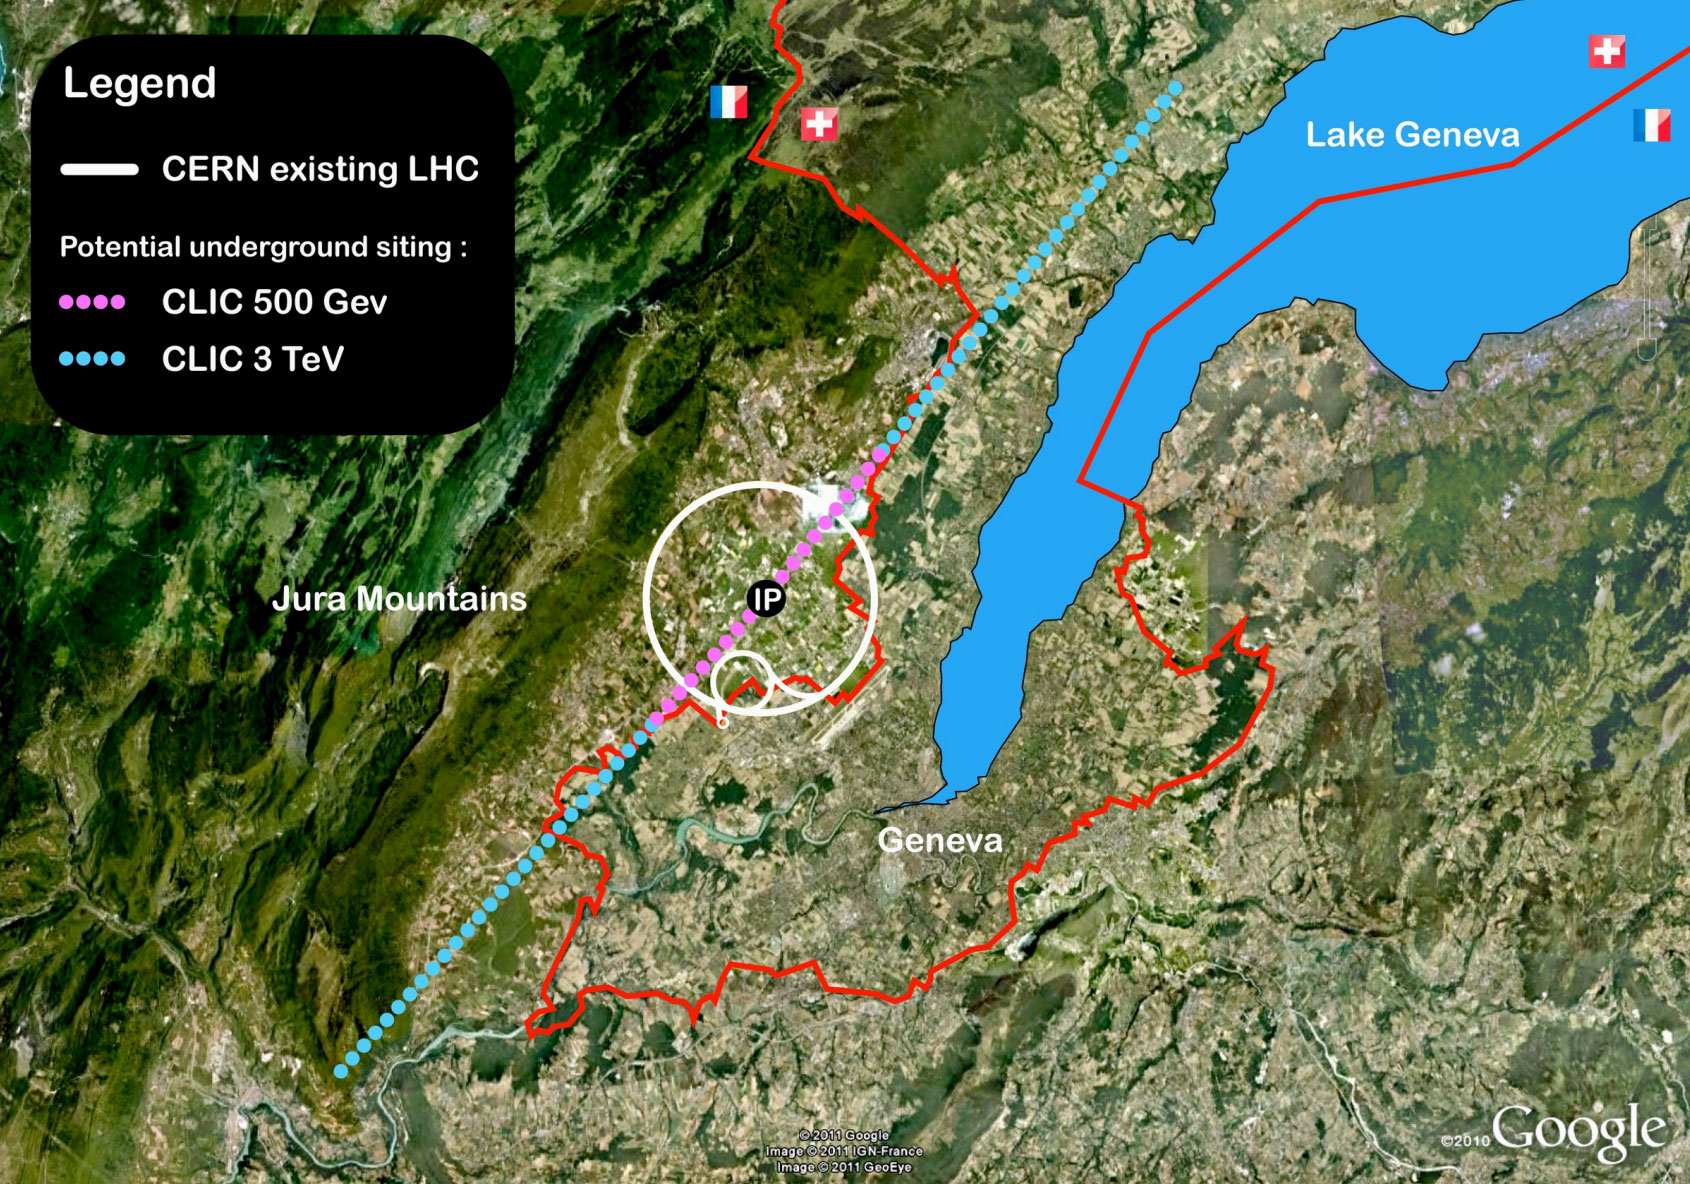
\includegraphics[width=1\textwidth,natwidth=1690,natheight=1184]{CLIC_Map.jpg}
\caption{Map Showing Potential Location for CLIC Accelerator Complex \cite{CLIC:Concept}}
\end{figure}

\paragraph{ILC/CLIC Location Comparison.}

The proposed locations for ILC and CLIC are shown to be feasible. However while the potential location for CLIC is merely conceptual, a great deal of research has gone into selecting the location for the ILC with a detailed analysis of potential sites.

The 2008 economic crisis led the US and UK to cut funds to the collider project and after the Great East Japan earthquake of 2011, Japan had an excess of reconstruction money which could be used for the ILC project indicating that Japan is most likely to host the ILC. In this case, the ILC will be located at Kitakami which has been shown to have geological advantages for construction and capable of providing good social facilities and transport links required. It would not make sense to build the ILC at CERN because CERNs priority for the next 20 years will be in exploiting the LHC at the higher energy range of 14 TeV. Also, it will be of international benefit to spread particle physics facilities across the world. Given the current economic climate of Europe, and the fact that Japan has offered to fund 50\% of the material costs of the ILC, Japan looks like the most likely location.
 
 
\subsubsection{Politics and Economics}

The construction of the next particle collider will depend on political decisions and the recognition of governments to fund it. Therefore it is important for governments to be involved as actively as possible and be kept informed of the project progress via FALC. However, scientific and political aspects of the project must be separated. While decisions regarding legal agreements, budget allocation and site selection for the next linear collider will be made by government agencies of participating nations, it is important that technical outlines and specifications are protected from any political compromises and are based solely on scientific facts. \cite{ILC:PIPReport}

For the ILC, the host country won't be finalised until around 2015 but with the current economic climate of Europe and the US, an international consensus is rapidly forming that Japan will host for the ILC. The global recession has meant that even the money needed for R\&D to finalise the design was tight \cite{Funding:Nature}.  With the estimated cost of \$7.8billion, the project has struggled to gain support from governments however the Japanese government has proposed to fund 50\% of the material costs, though the project will need international commitment in order to move forward.

Japan lost out in hosting the fusion reactor ITER in 2005 to France and has been looking for a world-class international science project since. The 2011 earthquake and tsunami in Japan gave rise to an excess of reconstruction funding, some of which could go towards a scientific project such as the ILC. The ILC has broad political backing in Japan with high profile politicians across the political parties supporting the project. This shows Japan's desire to play a more collaborative role in the global scientific community. \cite{Funding:NaturePress1}

The Japanese government budget proposal for the 2014 fiscal year includes an official budget for the ILC. Although a small amount,   $\sim$\$500k, it shows that the ILC is a recognised project of the Japanese government and is also the first official national budget for the ILC. The budget will be used to make a detailed study of the feasibility of an international framework for the ILC as a global project, as only after establishing international partnerships will Japan take the project further. \cite{LCC:Press4}
 
Currently the situation outside of Japan is as follows: countries are being contacted by Japanese government representatives to discuss possible contributions and a view of the ILC to be hosted in Japan has been integrated into the 2013 update of the EU strategy for HEP. If the ILC is approved in Japan, Europe will make a contribution. The US may be more reluctant to participate due to current budgetary constraints but the international diplomacy features of the project are sure to attract the US government's interest; a recent critical step is the positive inclusion of the ILC project in the US strategy for HEP \cite{Funding:NaturePress1, LCC:Press5}.
 
The ILC is more politically advanced in terms of attracting interest amongst governments compared to CLIC which doesn't yet have a technical design report or project implementation plan.
 
As well as the prestige of hosting a world-class science project, there will be long term economic benefits to the hosting region. The Japanese Productivity Centre calculated that the ILC could have a financial impact of over \$40 billion over a 30-year period and create 250,000 direct and indirect jobs \cite{Funding:SwissInfo}. The ILC facility will attract new businesses, for example, the technology spinoffs, which will boost the local and regional economies. No figures are available for CLIC but the economic benefits will be similar to ILC.